\documentclass[11pt,a4paper,UKenglish]{article}
\usepackage[utf8]{inputenc}           %% ... or latin1
\usepackage[T1]{fontenc,url}
\usepackage{textcomp,csquotes,varioref,graphicx}
\usepackage{gensymb}
\usepackage[english]{babel}

\usepackage[top=1in]{geometry}
\usepackage{float}
\usepackage[hidelinks,colorlinks]{hyperref} % trykkbar referering
\usepackage[all]{hypcap} % ref til starten av referansen
\usepackage{todonotes} % for kladd

\usepackage{marginnote}
\usepackage[backend=biber,style=numeric-comp]{biblatex}
\addbibresource{text_seg.bib}
% \addbibresource{bib.bib}


\title{UNIK4690 Project}
\author{
  Akhsarbek Gozoev  - akhsarbg \\
  Sadegh Hoseinpoor - sadeghh\\
  Key Lung Wong - keylw
}
\begin{document}
\newenvironment{loggentry}[2]% date, heading
{\noindent\textbf{#2}\marginnote{#1}\\}{\vspace{0.5cm}}
\newpage
\section*{Log}
\begin{loggentry}{19.04.18}{Week 1}
\begin{itemize}
  \item{Feedback on project proposal}
  \item{Overview of project}
    \begin{itemize}
     \item{simplification}
     \item{binary image $\rightarrow$ numbers $\rightarrow$ straight text $\rightarrow$ Classify}
   \end{itemize}
  \item{init; github - atom}
  \item{first test of charcter Segmentation}
\end{itemize}
\end{loggentry}


\newpage
\begin{loggentry}{26.04.18}{Week 2}
\begin{itemize}
  \item{Charcter Segmentation - Projection Histograms - OpenCV}
  \begin{itemize}
    \item{By projecting the histogram of the binary image on the Y-axis,
    we can find where the sentences/lines of text appears. Following, a
    projection histogram on the X-axis can discover where the charecters
    appear.}
  \end{itemize}

  \begin{figure}[H]
    \centering
    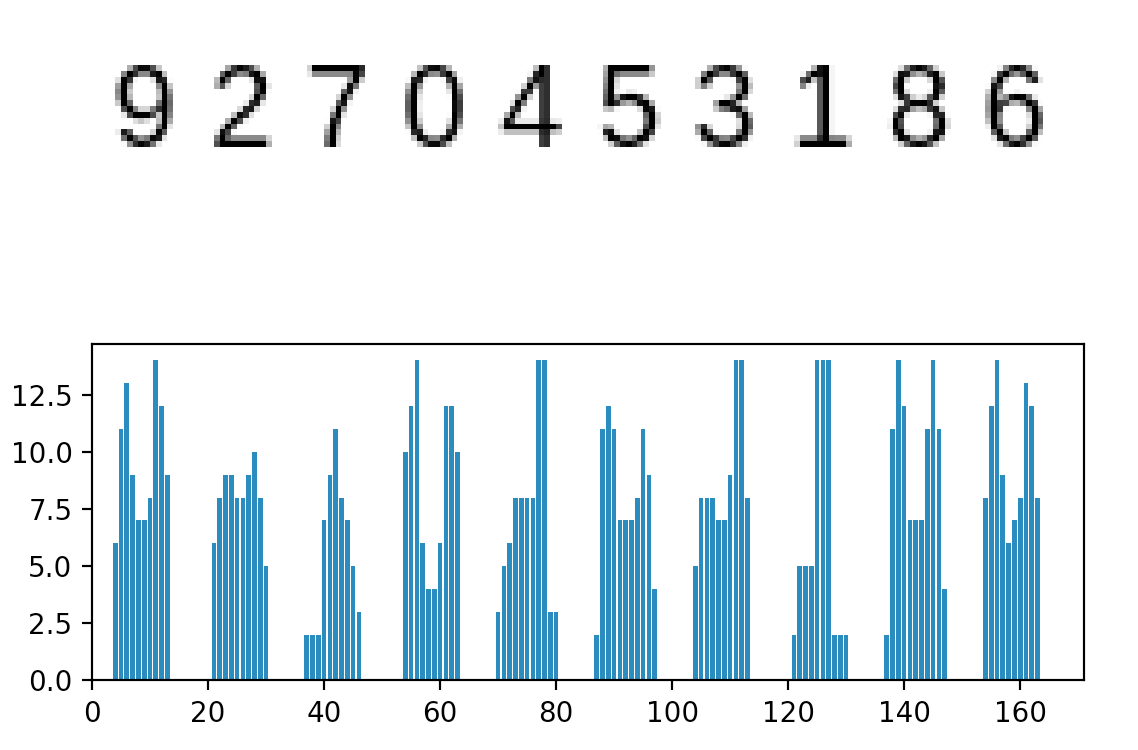
\includegraphics[height=4cm]{../res/0-9_segmented_out.png}
    \caption{[0-9] segmented with projection histogram}
    \label{fig:0-9_segmented_out}
  \end{figure}

  \item{Classification - Perceptron neural network - TensorFlow}
    \begin{itemize}
      \item{MNIST dataset - Datasett consisting of several thousand handwritten
      labeled numbers}
      \begin{itemize}
        \item{Numbers ranging from [0-9]}
        \item{Images are 28x28pixels}
      \end{itemize}
      \item{Hyperparameter tuneing}
      \begin{itemize}
        \item{Activation function}
        \item{Number of hidden layers}
        \item{Nodes in hidden layers}
        \item{Cost function}
        \item{Optimization function}
        \item{Learning rate}
      \end{itemize}
      \item{Theoretic accuracy of the network with 2 hidden layers ~98\%}
      \begin{itemize}
        \item{Measured accuracy ~97\%}

        \begin{figure}[H]
          \centering
          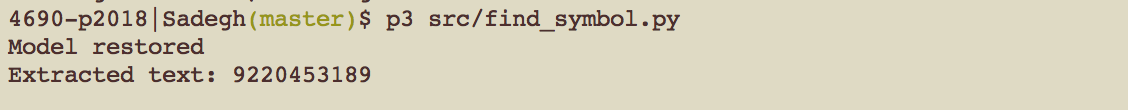
\includegraphics[height=1cm]{../res/classification_first_print.png}
          \caption{First output with classification. input see Figure ~\ref{fig:0-9_segmented_out}}
          \label{fig:classification_first_print}
        \end{figure}

      \end{itemize}
    \end{itemize}
\end{itemize}
\end{loggentry}


\newpage
\begin{loggentry}{03.05.18}{Week 3}
\begin{itemize}
  \item{Rotation of text}
  \begin{itemize}
    \item{Hough transform}
    \item{\textit{cv2.minAreaRect()}}
  \end{itemize}
  \item{How to distinguish between upside-down, and verticle vs horisontal text segments}
  \begin{itemize}
    \item{Classifiy in all 4 rotations, and choose the classification with highest avrage confidence}
  \end{itemize}
  \item{Classification - Perceptron neural network - Error}
  \begin{itemize}
    \item{Error rate too high, test-set accuracy 97\%, validation set accuracy $<$ 50\%}
    \item{CNN - TensorFlow Estimator API}
    \begin{itemize}
      \item{Challenging documantation; load/save models}
    \end{itemize}
    \item{Dataset - FNIST - Group contribution}
    \begin{itemize}
      \item{Dataset including several fonts}
      \item{English alphabet, and numbers [0-9]}
    \end{itemize}
  \end{itemize}
\end{itemize}
\end{loggentry}

\newpage
\begin{loggentry}{17.05.18}{Week 4}
\begin{itemize}
  \item{-----}
  \begin{itemize}
    \item{-----}
    \item{-----}
  \end{itemize}
  \item{------}
\end{itemize}
\end{loggentry}

\end{document}
